\documentclass[tikz,border=4pt]{standalone}
\usetikzlibrary{arrows.meta,positioning}
\begin{document}
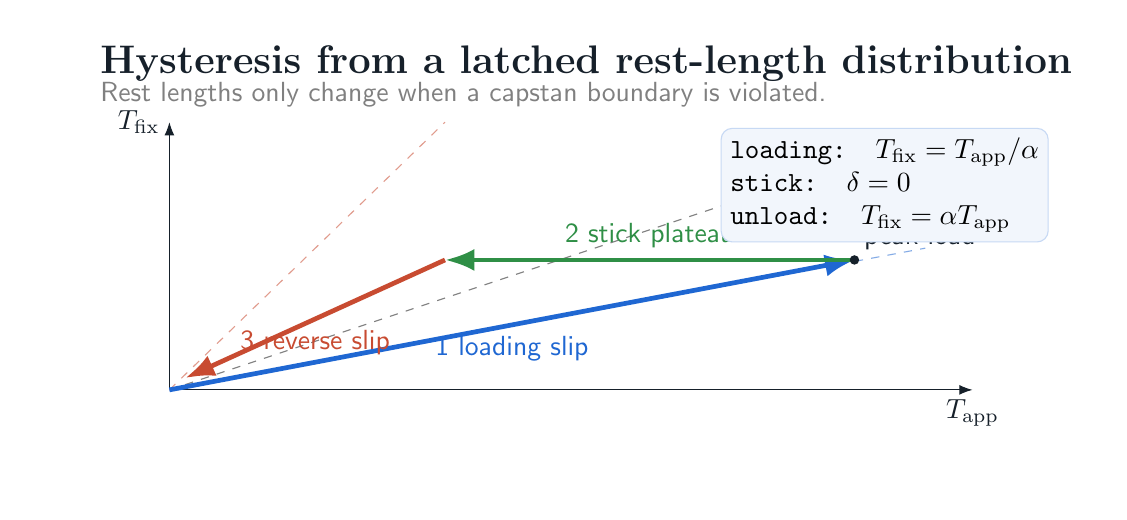
\begin{tikzpicture}[>=Latex, font=\sffamily]
  \definecolor{ink}{HTML}{16202A}
  \definecolor{blue}{HTML}{1F67D2}
  \definecolor{green}{HTML}{2F8F46}
  \definecolor{red}{HTML}{C84B31}
  \draw[fill=white, draw=none] (-0.8,-0.9) rectangle (12.8,5.0);
  \node[anchor=west, font=\bfseries\Large, text=ink] at (0,4.55) {Hysteresis from a latched rest-length distribution};
  \node[anchor=west, text=gray] at (0,4.15) {Rest lengths only change when a capstan boundary is violated.};
  \draw[->, ink] (1,0.4) -- (11.2,0.4) node[below] {$T_{\rm app}$};
  \draw[->, ink] (1,0.4) -- (1,3.8) node[left] {$T_{\rm fix}$};
  \draw[gray, dashed] (1,0.4) -- (10.6,3.6);
  \draw[blue!55, dashed] (1,0.4) -- (10.6,2.2);
  \draw[red!55, dashed] (1,0.4) -- (4.5,3.8);
  \draw[->, blue, line width=1.7pt] (1,0.4) -- (9.7,2.05) node[midway, below] {1 loading slip};
  \draw[->, green, line width=1.7pt] (9.7,2.05) -- (4.5,2.05) node[midway, above] {2 stick plateau};
  \draw[->, red, line width=1.7pt] (4.5,2.05) -- (1.2,0.55) node[midway, below] {3 reverse slip};
  \fill[ink] (9.7,2.05) circle (0.06) node[above right] {peak load};
  \node[draw=blue!25, fill=blue!6, rounded corners, anchor=west, align=left, font=\ttfamily] at (8.0,3.0)
    {loading: $T_{\rm fix}=T_{\rm app}/\alpha$\\stick: $\delta=0$\\unload: $T_{\rm fix}=\alpha T_{\rm app}$};
\end{tikzpicture}
\end{document}
